\documentclass[twocolumn]{article}
\usepackage{graphicx}
\usepackage{float}
\usepackage[backend=biber,url=false,doi=true]{biblatex}
\addbibresource{crosby\_491\_paper\_draft.bib}
\title{Circgraph: a Galaxy tool for Circos-enabled genomic data visualization}
\author{Stephen Crosby}
\begin{document}
\maketitle
\section*{Abstract}
Advancements in molecular biology in the past two decades have led to the acquisition of
unprecedented amounts of DNA sequence data, but the visualization of this data and its
interpretation remain important challenges to the scientific community. Several approaches to
create informative plots of sequence data have been devised in response to these challenges, 
including Circos: graphics software which allows users to design circular plots highlighting
interesting genomic features and comparing different organismal genomes. In order to facilitate sequence analyses and Circos plot development, an online Galaxy tool was developed which
will enable scientists to incorporate bioinformatics techniques into their work while bypassing the learning curve associated with command-line tool usage. The tool, which has both command-line and web-based interfaces, allows users broad cosmetic control over the appearance of produced Circos plots, includes methods for parsing and interpreting several common file types used for visualizing genomic data, and supports most the principal track types present in the Circos suite. This new interface to the existing Circos software will enable life scientists to easily and efficiently create informative views of a variety of sequence data formats.

\section*{Introduction}
Macromolecular sequencing has been the underpinning of many crucial developments in modern biomedical research, and since the advent of sequencing technology in the 1970s, improvements in experimental techniques have enabled scientists to produce ever-increasing amounts of nucleic and amino acid sequence data. The increasing popularity of these high-throughput molecular techniques has challenged the bioinformatics community to develop new solutions for data-management, statistical analysis, and genome annotation. Visualizing this newly produced genomic data remains an important obstacle to both the effective utilization of sequence data as well as the continued growth and adoption of bioinformatic methods by new scientists. Effectively managing the scale at which sequence data are visualized is critical to forming insightful conclusions, as biologically interesting genomic phenomena can occur at the single-codon or whole genome levels. Visualization efforts are fraught with other problems as well; the emergence of new file formats to handle increasing amounts of data necessitates constant development and support to ensure existing applications retain their utilities.

Naturally, a wide variety of visualization software has been produced as sequencing efforts have grown simultaneously more popular and successful; these programs in general represent sequence data as a variety of separate, static windows depicting linear chromosomes joined together by linear links indicating homologous regions as well as classic visualization options like line plots and tables. The programs often use color to encode numerical information about the uncertainty of the identity of a nucleotide within a genome and thereby maximize the information density of a single view. These softwares offer different options for scaling and filtering data to address the difficulties heretofore described. Of the several responses which have made to the challenge of visualization, one of the most successful has been Circos: a software suite produces circular analogs of classical graphics and promises to facilitate the comparison of genomes with two-dimensional data tracks and links. One of the core aims of Circos is to facilitate the analysis of genomic data by allowing scientists to create vast diagrams conveying information at several levels of specificity. Although the software has been successfully used to produce figures in leading scientific journals and in its pioneering study was applied to genomic datasets spanning several orders of magnitude (kbp to Gbp), the creators of the software caution that figure quality is closely associated with aesthetic decisions made by scientists deciding which data they seek to convey, indicating that the software still has room for improvement as an exploratory visualization tool. Other visualization tools such as Circoletto, which pairs the Circos visualization paradigm with BLAST sequence identity results, have attempted to improve on Circos' visualization capabilities. 

Beyond the difficulties intrinsic to the analysis of this newly obtained high-throughput data, another obstacle to the growth of bioinformatics within classical scientific disciplines is the learning curve associated with the use of these new, computerized tools; 21st century software development initiatives such as the Galaxy project are lowering the barriers between established wet-lab scientists and cutting edge computational techniques by eschewing the traditional command-line interface in favor of broadly-accessible, user-friendly web apps. A wide variety of bioinformatics tools and workflows have been made publicly available in the wake of the discpline's increasing popularity, and open-source tools present low financial barriers to life scientists in academia; however, much open-source software is tailored to power users on *NIX operating systems with a great deal of command line experience. These individuals make up only a subset of the total potential userbase for new analytical software, highlighting the need for solutions which support a wide variety of operating systems and present little learning curve. An assortment of online services have been developed in order to address this issue and improve the accessibility of bioinformatics solutions to the scientific community at large. The Galaxy Project is a collection of bioinformatics tools administrated principally by scientists at Johns Hopkins and Penn State, but other developers are free to create their own scripts and make them publicly available. The central initiative of the project -- to put bioinformatics software in the hands of capable scientists with the expertise to ask difficult questions and make subtle inferences about genomic data -- was the principal factor motivating the development of Circgraph. The Circgraph Galaxy tool replicates much of the core functionality of the Circos software suite while adding minimal support for parsing data types common to biochemical sequence analysis, and its main contribution to the body of scientific knowledge is that the program will make the existing Circos software more readily accessible to life scientists by creating configuration files from a point-and-click user interface automatically.  


\section*{Methods}
Developed in 2004, the Circos visualization software suite manages the creation of circular plots of genomic datasets using text-based configuration files; with a specific format analogous to the XML standard, configuration files have the potential to be extensibly generated by exploiting existing software. Much like an xml file, a general Circos configuration file is composed of blocks which correspond to objects ranging from heatmaps and scatterplots to position- and parameter-dependent formatting rules. Within the blocks are parameters specifying cosmetic options and indicating the data files with which data-dependent tracks will be populated. Beyond these ordinary parameters, whose possible values are well-defined within the Circos specification, objects can be customized by user-created rules. These rules, which rely on Perl code inserted directly into the configuration file, conditionally modify parameter values and vastly expand user control over the final diagram.  

An XML-driven Galaxy tool through which users can specify data to be used in tracks and cosmetic parameters for the Circos plots was developed with Jinja2, and the core of the new Galaxy tool is a Python script which manages these parameters and writes them to configuration files consistent with the Circos specification. Currently, the Circgraph workflow is a two-stage process in which a user specifies options and quickly generates a template xml file to be passed to a command-line interface. At the command line, the user specifies data files and parameters relevant to link creation and then must manually call Circos in order to produce diagrams. User data is parsed into the appropriate format specified for Circos plots, but no further effort is made to store the data for ad hoc analyses or real-time calculations.

\section*{Results and Discussion}

In order to facilitate the visualization of high-throughput genomic data in several file formats, Circgraph, a web-based Galaxy tool exploiting the existing Circos software suite freely available online, was developed. Currently, the program has been implemented as a command-line tool in order to allow the user to pass data files dictating the composition of data tracks, but the software support required for users to set parameter values from the online Galaxy interface has already been developed.

Circgraph can accept and parse several common genomic file types including fasta, bigWig, gff3, and ProgressiveMauve backbone files into text files suitable for interpretation by Circos. In particular, fasta files are used to drive the creation of the karyotype and specify the chromosomes to be represented in the plots, while bigWig files are parsed into two-dimensional data tracks such as heatmaps, histograms, or scatterplots. The current Circgraph implementation does not capture the full complexity of the gff3 datatype but can parse feature locations into highlights. Alignments in general are best represented by links within the Circos visualization scheme, and consequently, ProgressiveMauve backbone files containing multiple sequence alignment data are parsed into link files that illustrate connections between regions of sequence homology.  

As previously discussed, Circgraph handles several of the principal data track types available through Circos including 2D data tracks such as heatmaps, histograms, and scatterplots, highlights indicating specific regions of interest within sequence data, and links associating homologous runs within two sequences. Each of these fields can be customized with a wide variety of cosmetic parameters dictating the scales of the objects to be represented as well as their orientations, colors, and relative positions within the Circos figure. 

\begin{figure}
\centering
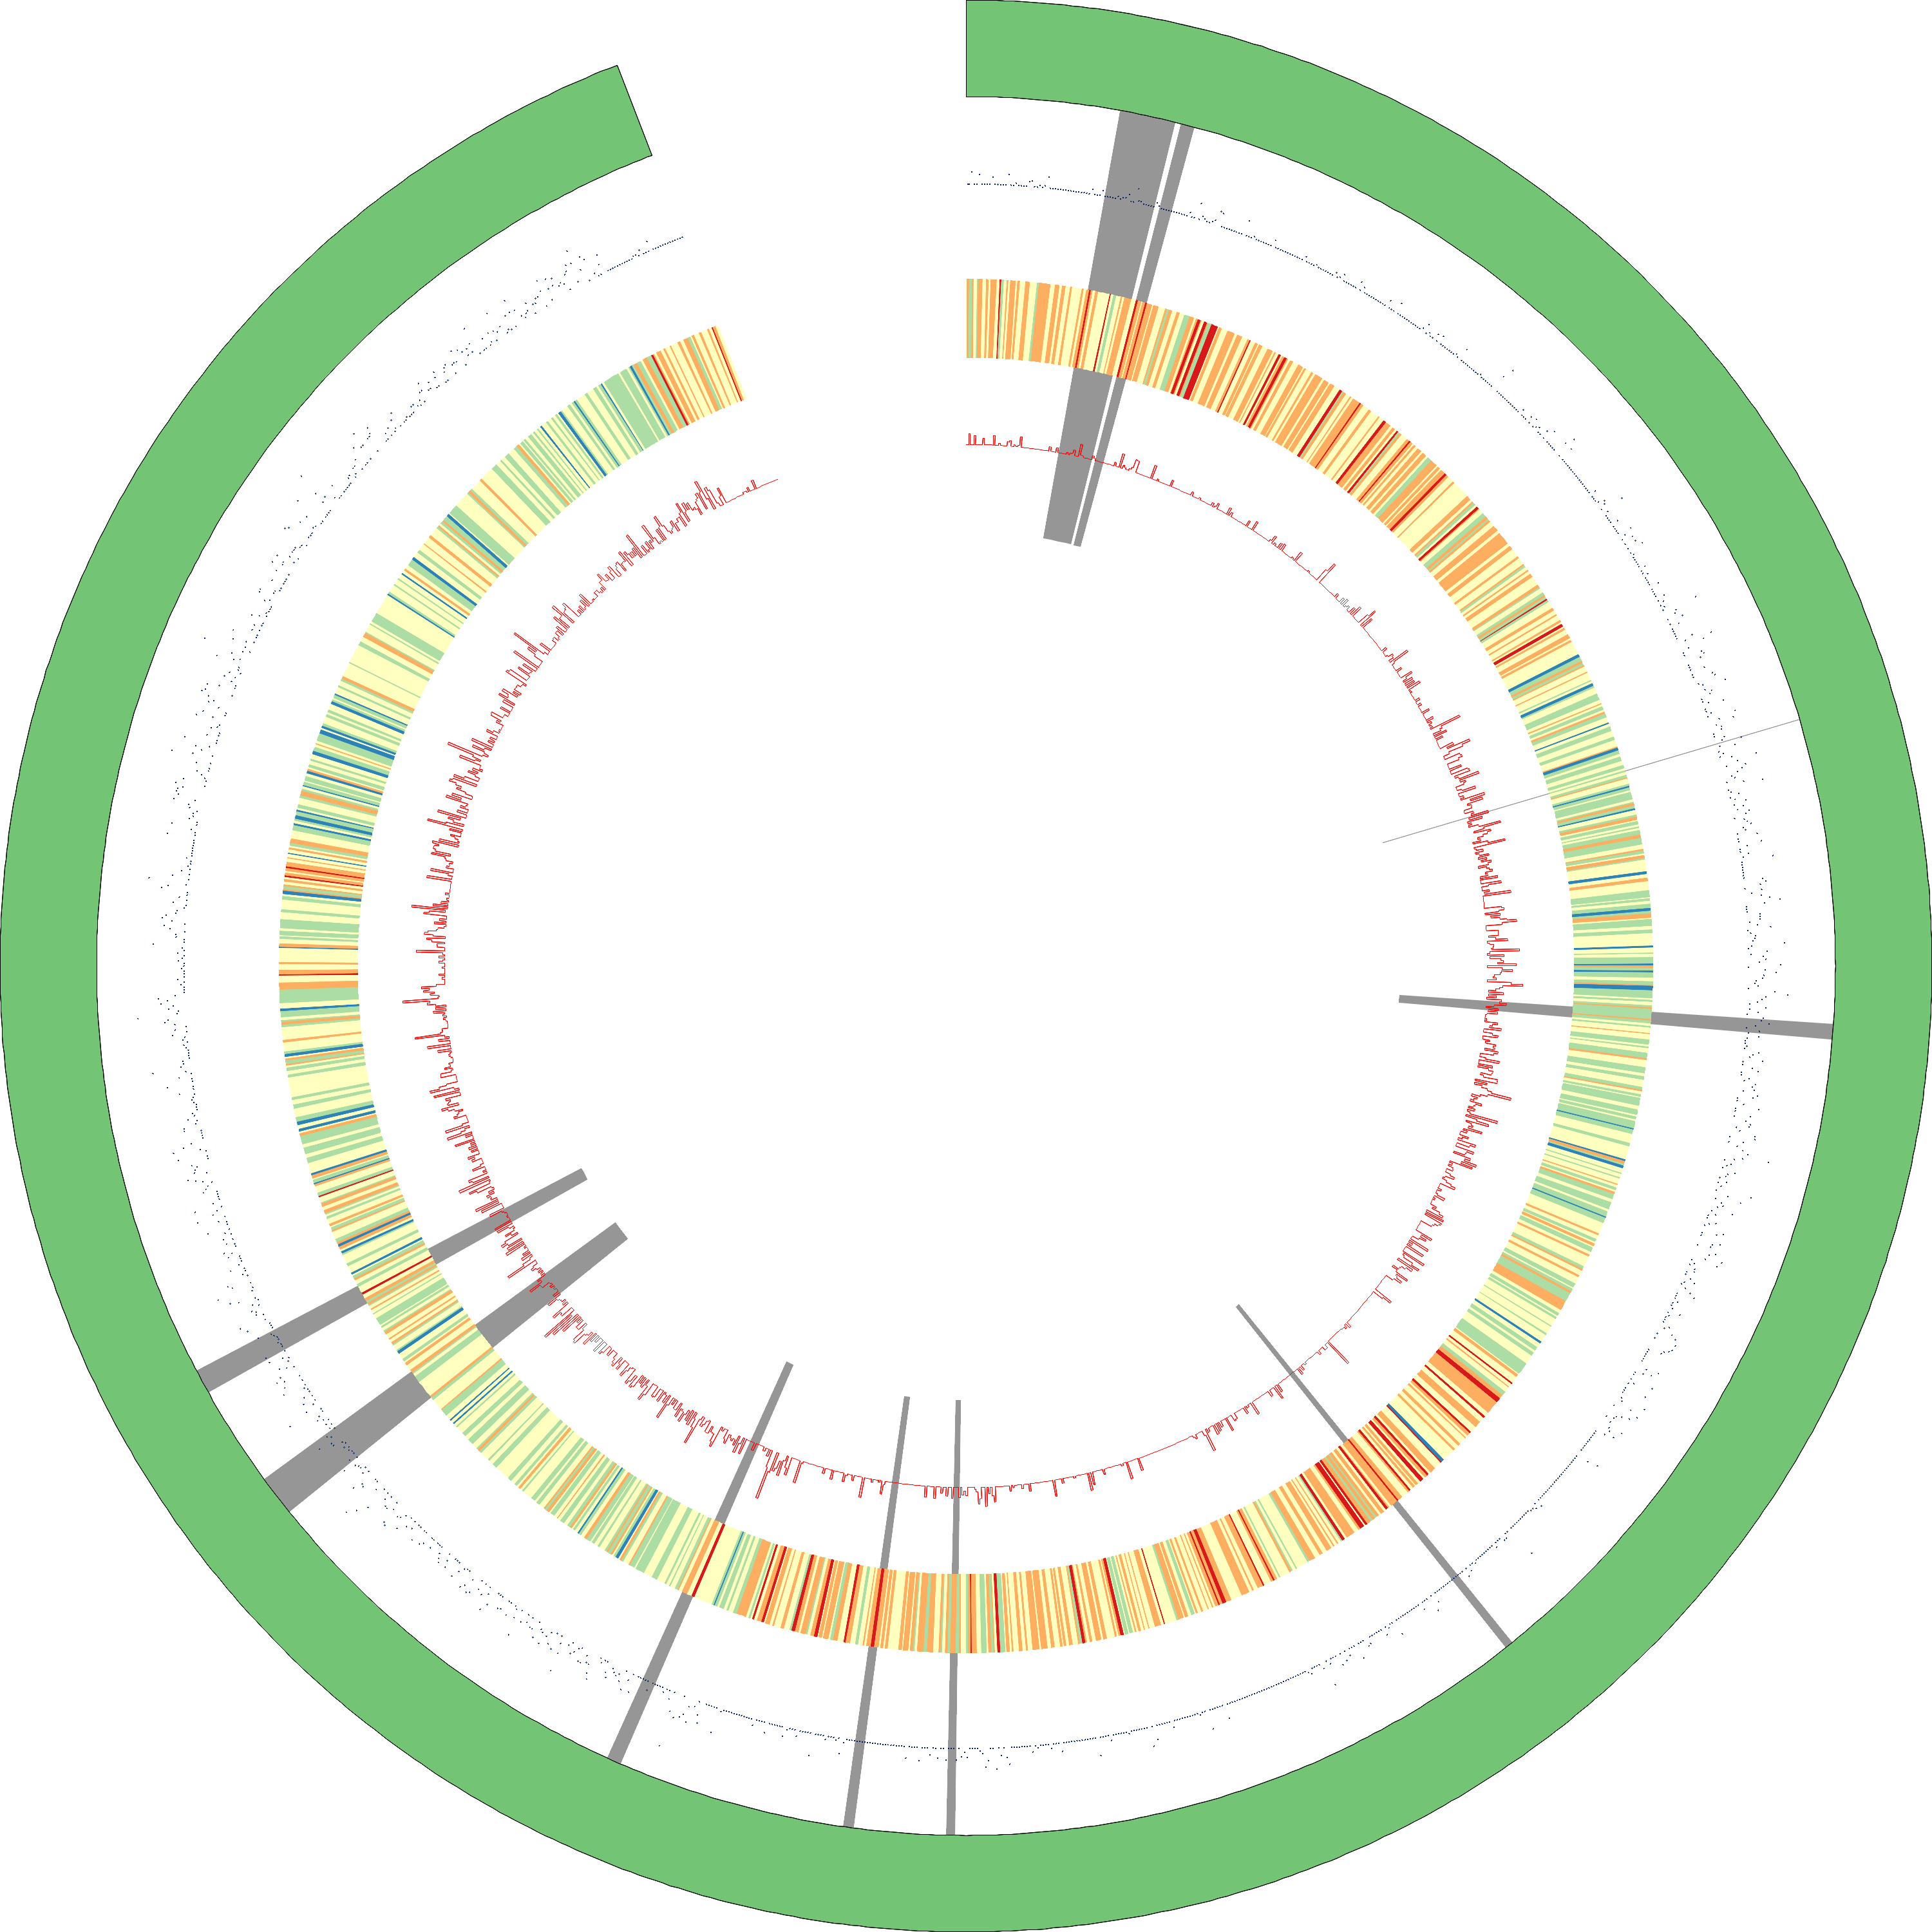
\includegraphics[scale=0.1]{./results/hilite.png}
\caption{Circgraph allows users to create several native Circos data track types, including histograms, heatmaps, and scatterplots. Highlights can also be added to accentuate certain regions; here, highlights are shown in grey.}
\end{figure}

\begin{figure}
\centering
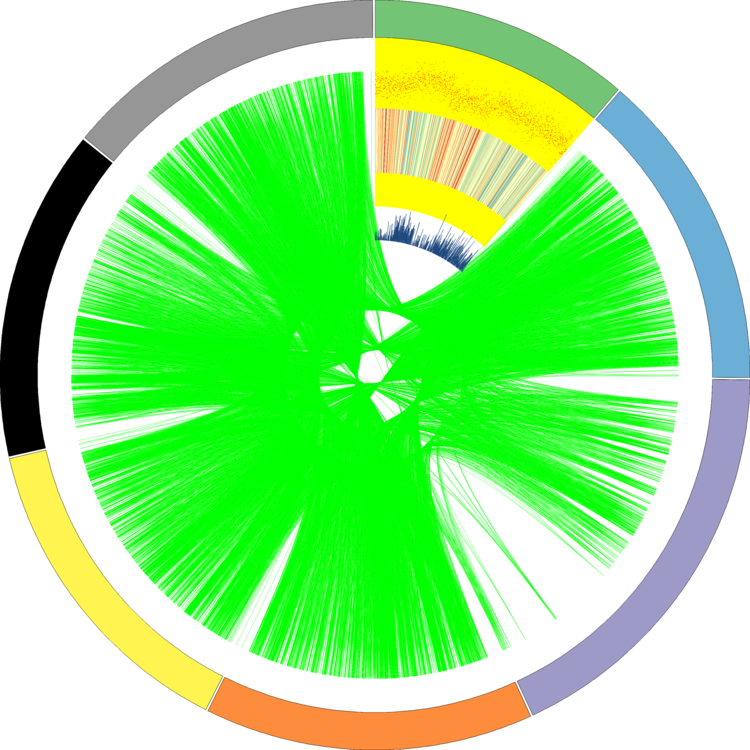
\includegraphics[scale=0.1]{./links.png}
\caption{Circgraph supports arrangement of multiple chromosomes within a plot and can create links between chromosomes if provided with ProgressiveMauve-generated backbone files.}
\end{figure}

Several challenges remain to the effective use of Circos for genomic data visualization; in particular, continuing improvements to existing algorithms and workflows which can separate statistically-significant, biologically-relevant data from the ambient dataset will improve the signal-to-noise ratio of Circos plots. Aside from the two-dimensional data tracks, links are the principal representative element of a Circos diagram and suggest homology between sections of the organismal genome. While proposing to maximize the '`information-to-ink" ratio of a genomics figure, the Circos software suite cannot compensate for an entirely naive approach to bioinformatics analysis; cluttered diagrams can prevent scientists from drawing inferences (Figure 3) or could even mask the data itself. Although internal parameters and extensive user customization with the use of rules can enable scientists to create compelling narratives from computational analyses, determining the extent to which data supports a particular narrative, if any, is the principal problem associated with genomics visualization. Whether these analytical judgements can be made without the scientist's supervision is a question that remains to be answered.

\begin{figure}
\centering
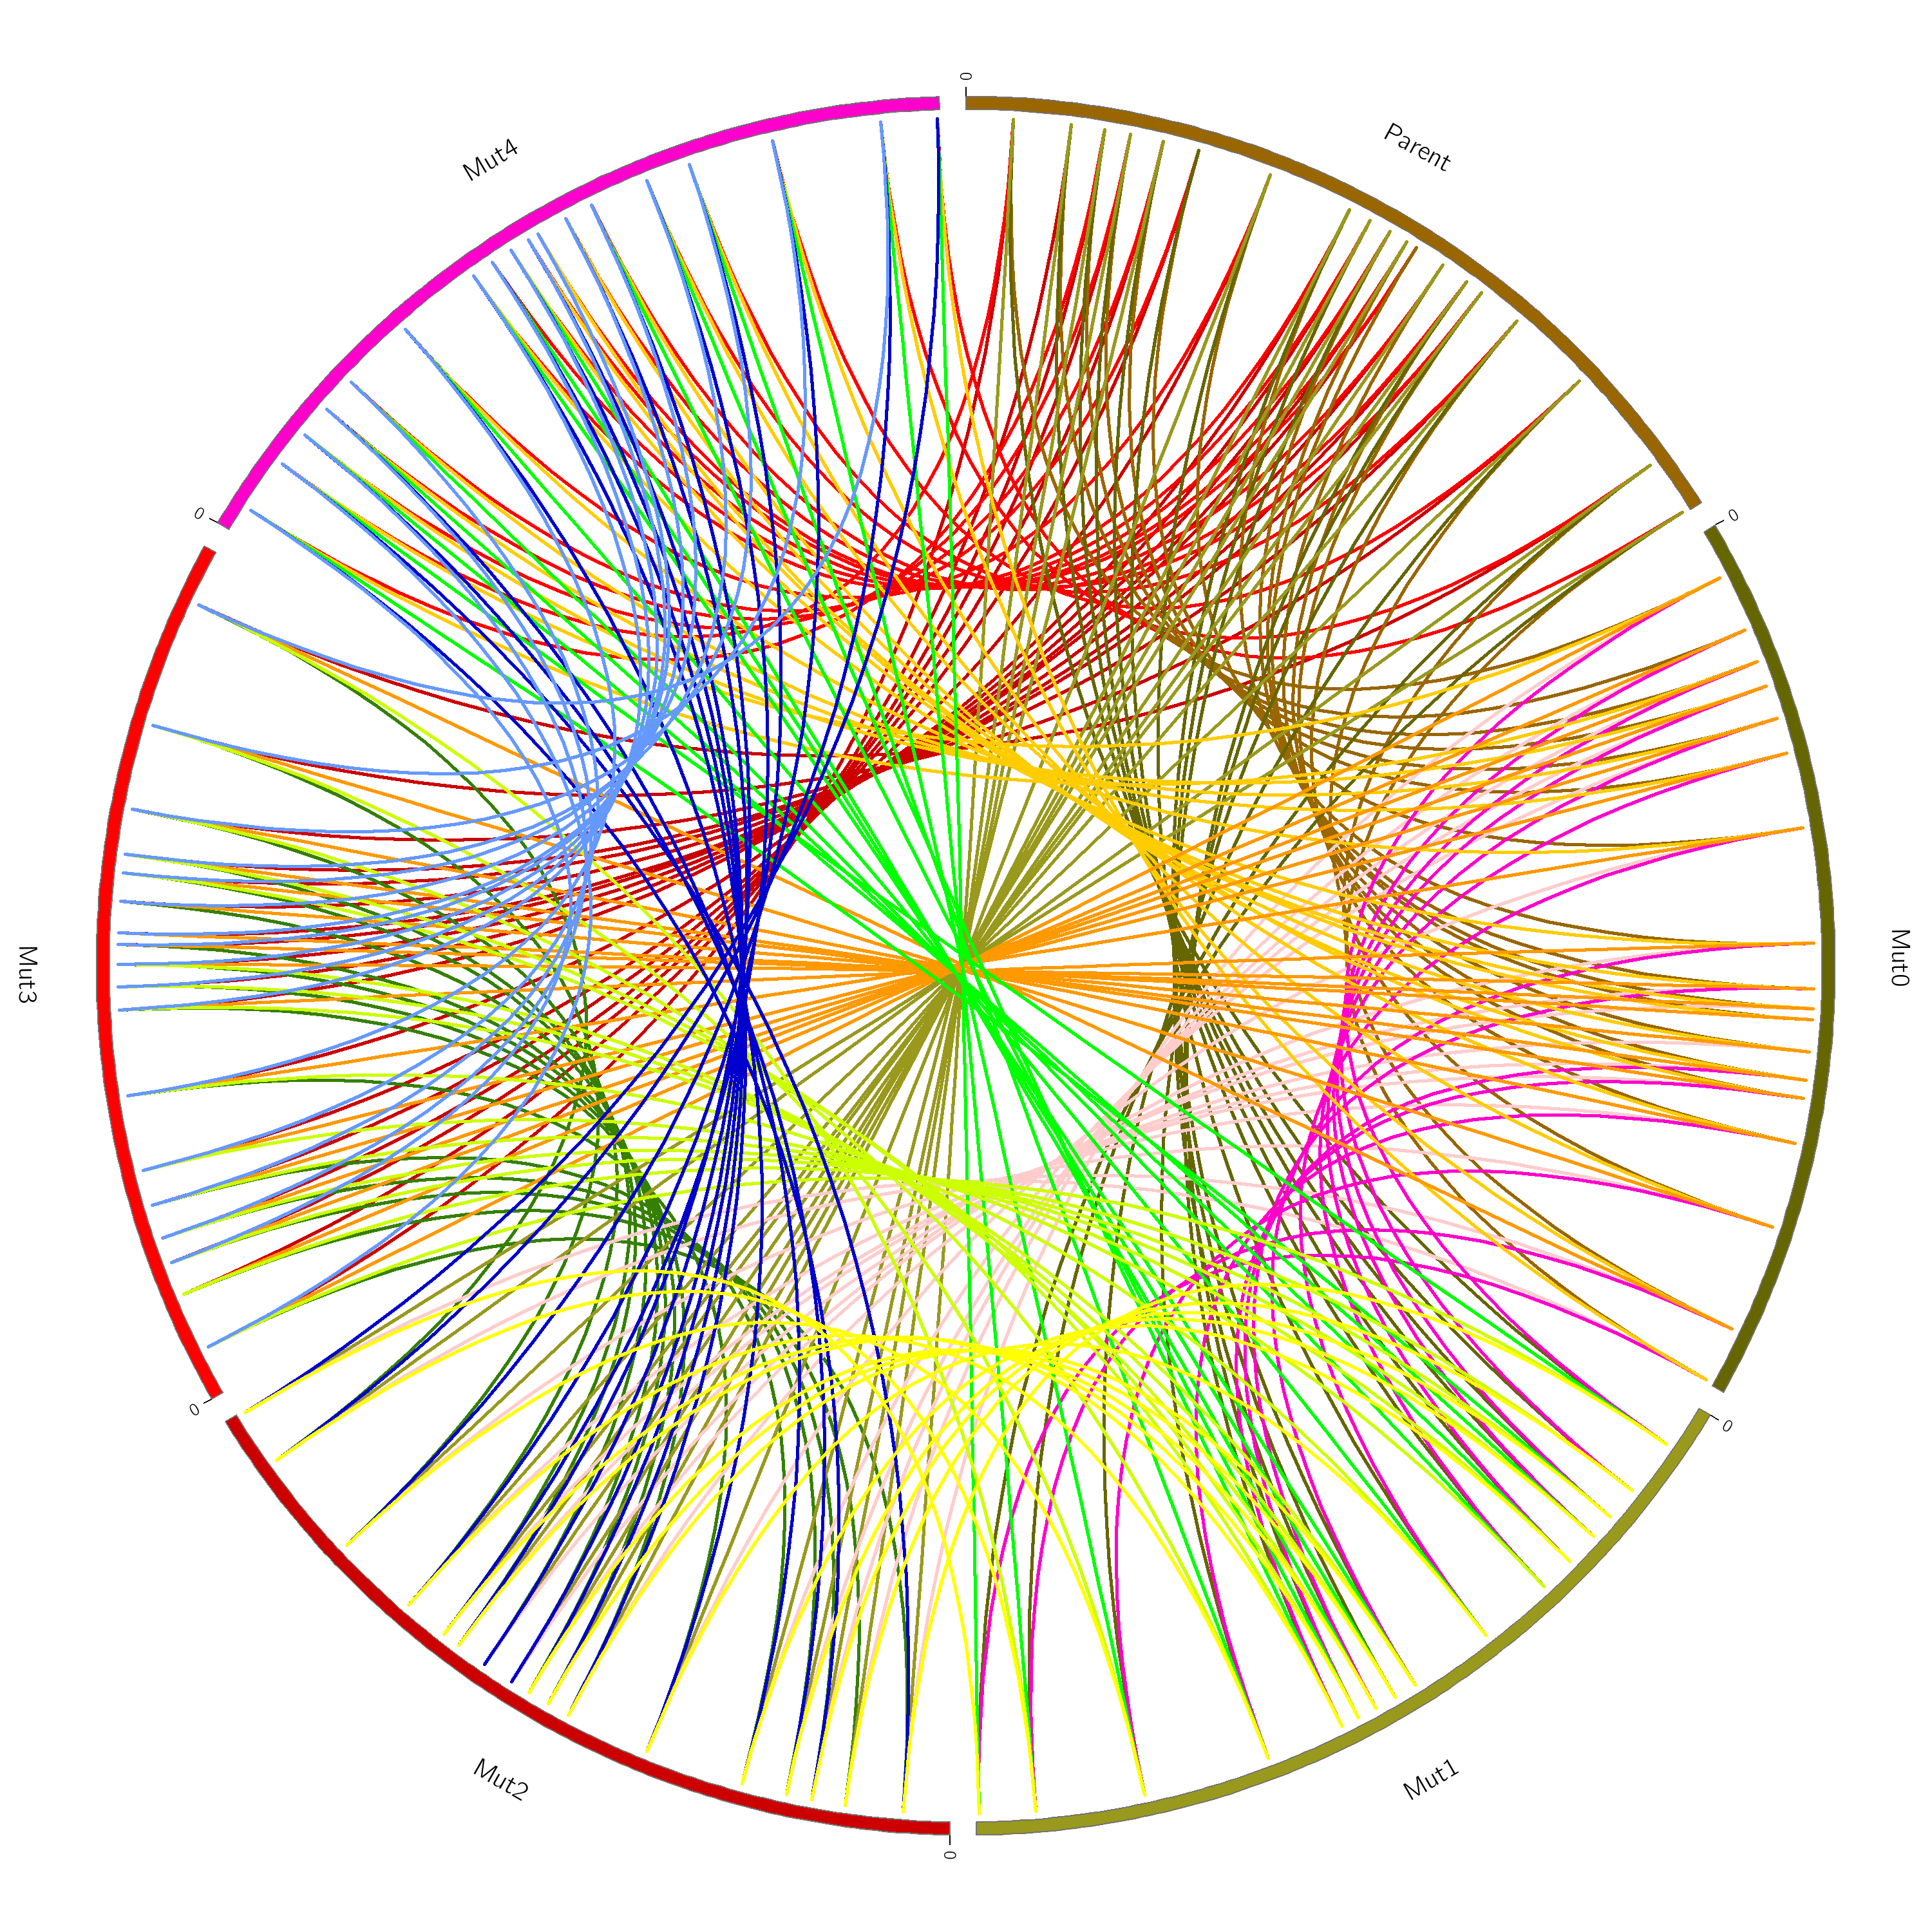
\includegraphics[scale=0.1]{./Generated_Data_Non_Ribbon.png}
\caption{Even when color-coded, unstratified link data is not suitable for creating easily interpreted graphics. Currently, Circgraph does not support rules for data stratification as the graphic is being created.}
\end{figure}

\begin{figure}
\centering
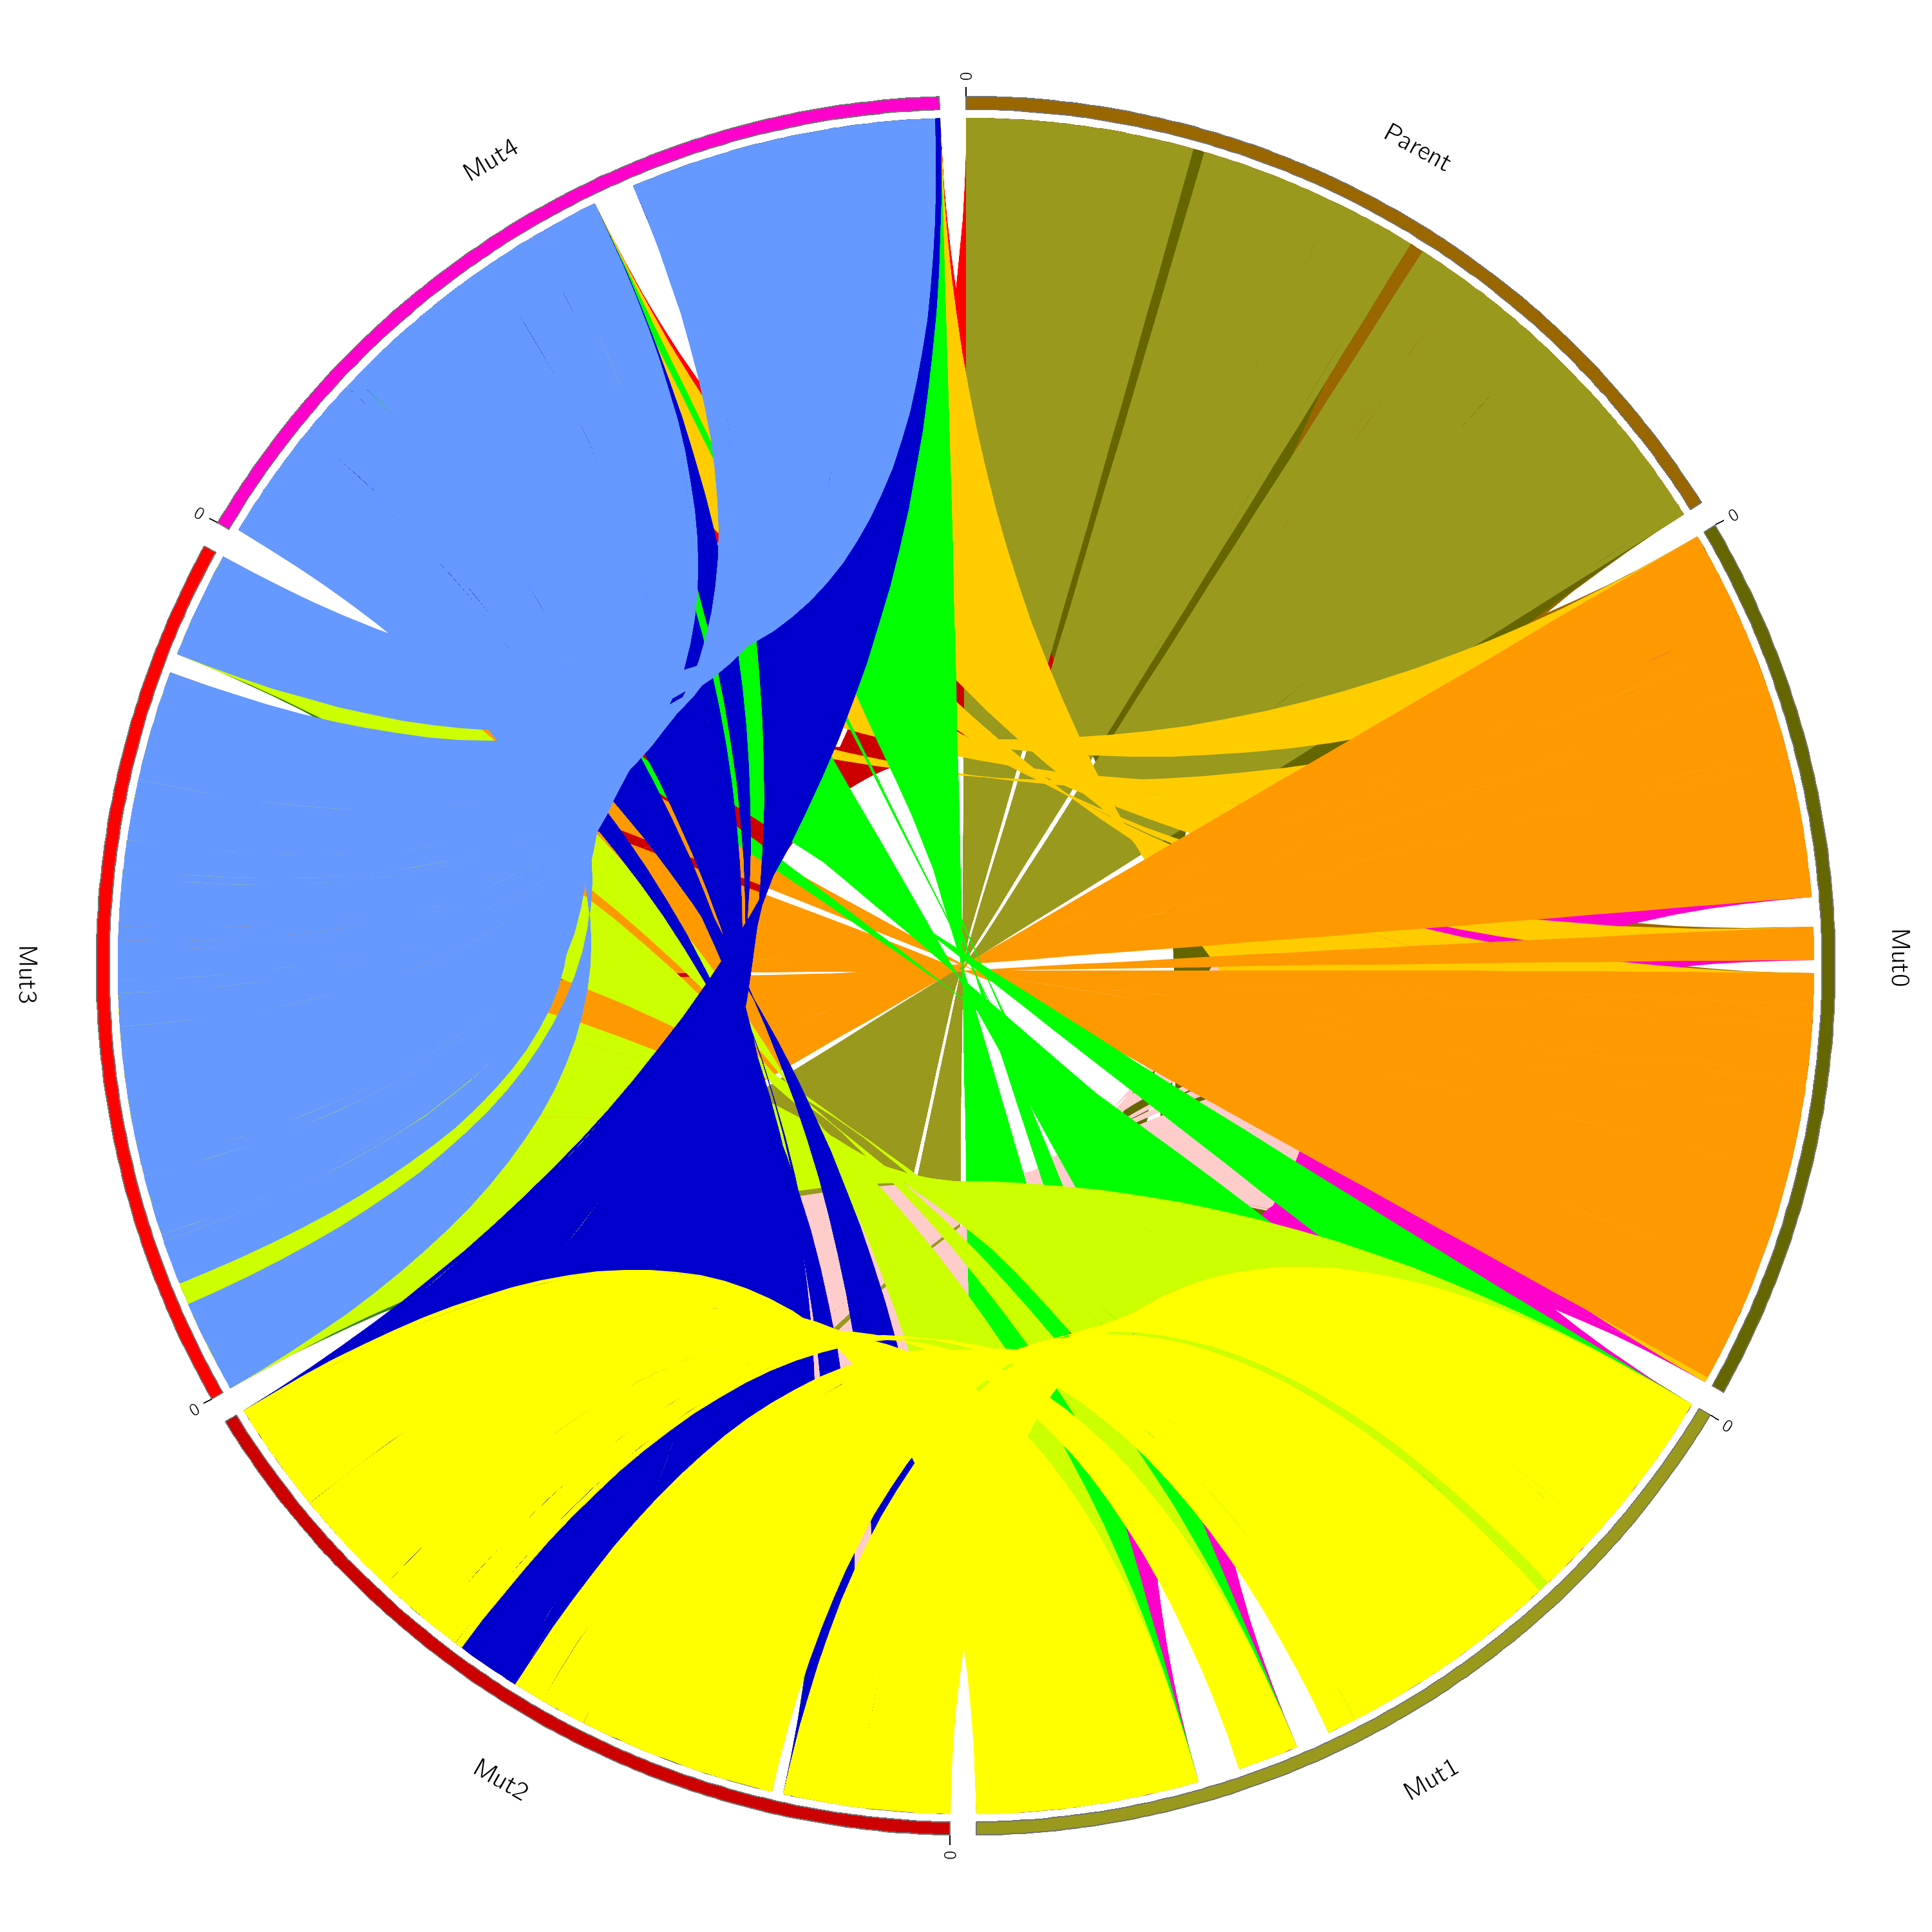
\includegraphics[scale=0.1]{./Generated_Color_Fixes.png}
\caption{Coarser link data poses its own interpretive difficulties; larger, opaque ribbon links can obscure each other.}
\end{figure}

Continued development of Circgraph will be required in order to capture the full span of features offered by the Circos visualization software, and guided, intelligent creation of high-quality graphics may be possible with additional code improvements. This edition of Circgraph includes several data plotting capabilities, but the inclusion of rules -- single lines of Perl code which dictate formatting on the fly based on the contents of data files -- greatly compounds the customizability of graphs the software can produce. However, incorporating these dynamic formatting options into the Circgraph tool without introducing a programming learning curve could be a challenge, as only supporting a subset of Circos' Perl capabilities directly limits the types of questions scientists could use the software to answer. Additionally, although elements of the software allowing users to view their data at different scales are in the process of being implemented, no exploration of the effects varying scale could have on interpretability has been done. Automatic detection of sensible formatting options and determination of the optimal scale at which the data should be visualized are issues which could be addressed alongside the addition of more extensive Circos features in subsequent releases of the Circgraph Galaxy tool.

\section*{References}
\printbibliography

\end{document}
